\documentclass[11pt,reqno]{amsart}

% --- Encoding / fonts ---
\usepackage[T1]{fontenc}
\usepackage[utf8]{inputenc}

% --- Core AMS packages ---
\usepackage{amsmath,amssymb,amsfonts,amsthm,mathtools}

% --- Graphics and lists ---
\usepackage{graphicx}
\usepackage{enumitem}


% --- Hyperref (load late) ---
\usepackage[pdfencoding=auto,psdextra]{hyperref}

% --- Page layout ---
% amsart already has a well-tested layout.
% If you must change margins, keep geometry simple:
\usepackage[a4paper,margin=3cm]{geometry}

% --- Theorem environments (single consistent system) ---
\theoremstyle{plain}
\newtheorem{theorem}{Theorem}[section]
\newtheorem{lemma}[theorem]{Lemma}
\newtheorem{proposition}[theorem]{Proposition}
\newtheorem{corollary}[theorem]{Corollary}

\theoremstyle{definition}
\newtheorem{definition}[theorem]{Definition}
\newtheorem{example}[theorem]{Example}
\newtheorem{question}[theorem]{Question}
\newtheorem{conjecture}[theorem]{Conjecture}

\theoremstyle{remark}
\newtheorem{remark}[theorem]{Remark}
\newtheorem{claim}[theorem]{Claim}
\newtheorem{assertion}[theorem]{Assertion}
\newtheorem{notations}[theorem]{Notations}
\newtheorem{assumption}{Assumption}
\newtheorem{hypothesis}{Hypothesis}

\newtheorem*{theoremA}{Theorem A}
\newtheorem*{theoremB}{Theorem B}
\newtheorem*{theoremC}{Theorem C}

% --- Operators ---
\DeclareMathOperator{\IFS}{IFS}
\DeclareMathOperator{\diam}{diam}
\DeclareMathOperator{\vol}{vol}

% --- TOC depth ---
\setcounter{tocdepth}{3}

% --- Title & Authors ---
\title[Transverse Blowout and Laminar First Passage]{Transverse Blowout, Laminar First Passage, and Stability Indices in Monotone Skew Products}

\author[F. H. Ghane]{Fatemeh Helen Ghane}
\address{Department of Pure Mathematics, Ferdowsi University of Mashhad, Mashhad, Iran}
\email{htina@um.ac.ir}

\author[M. Zaj]{Marzie Zaj}
\address{Department of Pure Mathematics, Ferdowsi University of Mashhad, Mashhad, Iran}
\email{zaj@ferdowsi.um.ac.ir}

\thanks{Corresponding author: F. H. Ghane (\texttt{htina@um.ac.ir})}

\keywords{ Monotone skew products, blowout bifurcation, on--off intermittency, laminar first passage, riddled basins, stability indices, thermodynamic formalism, multifractal spectra.}
\subjclass[2020]{Primary 37D25; Secondary 37A35, 37C40, 37A60.}

\begin{document}

\maketitle


\begin{abstract}

\end{abstract}


\section{Active oscillator--actuator model}

Active vibration control combines structural sensing, feedback control,
and force actuation to modify the dynamic response of lightly damped
mechanical structures. Direct velocity feedback is widely used because of
its simplicity and effectiveness in reducing resonant vibrations
\cite{Balas1979,Preumont2018,Hirschfeldt2025}. In practical
implementations, however, actuators possess finite bandwidth and internal
dynamics, which may substantially modify the stability of the closed-loop
system \cite{GohCaughey1985}. Moreover, actuator nonlinearities may
produce self-excited oscillations and limit cycles
\cite{DalBorgo2020}.

Motivated by these observations, we consider the reduced-order
oscillator--actuator model

\begin{equation}
\label{eq:model}
\begin{aligned}
\dot x &= v,\\
\dot v &= -\omega_0^2x-(d-g)v+f,\\
\tau\dot f &= k_sx-f-\kappa x^2.
\end{aligned}
\end{equation}

Here $x$ denotes the modal displacement,
$v=\dot x$ the modal velocity,
and $f$ the actuator force per unit modal mass.
The parameter $\omega_0>0$ is the natural frequency of the uncontrolled
structure,
$d>0$ is the passive damping coefficient,
$g$ is the velocity-feedback gain,
$\tau>0$ is the actuator time constant,
and $k_s$ is the linear stiffness-compensation gain.
The coefficient $\kappa\neq0$ represents the leading nonlinear actuator
distortion.

The actuator equation corresponds to the first-order tracking law

\[
\tau\dot f+f=f_c(x),
\qquad
f_c(x)=k_sx-\kappa x^2.
\]

When

\[
k_s=\omega_0^2,
\]

the actuator exactly compensates the structural stiffness, recovering the
standard actuator model considered in active vibration control.
The parameter $k_s$ is introduced here because it provides a natural
second unfolding direction for the zero--Hopf singularity.

The equilibrium points satisfy

\[
v=0,
\qquad
f=\omega_0^2x,
\]

and therefore

\[
(k_s-\omega_0^2)x-\kappa x^2=0.
\]

Hence

\[
x=0
\]

or

\[
x=\frac{k_s-\omega_0^2}{\kappa}.
\]

At the critical value

\[
k_s=\omega_0^2,
\]

these two equilibria coalesce, and the unique equilibrium is

\[
E_0=(0,0,0).
\]

The Jacobian matrix at $E_0$ is

\[
A=
\begin{pmatrix}
0&1&0\\
-\omega_0^2&g-d&1\\
k_s/\tau&0&-1/\tau
\end{pmatrix},
\]

whose characteristic polynomial is

\[
p(\lambda)
=
\lambda^3+
\left(d-g+\frac1\tau\right)\lambda^2+
\left(\omega_0^2+\frac{d-g}{\tau}\right)\lambda
+\frac{\omega_0^2-k_s}{\tau}.
\]

Therefore the origin is a zero--Hopf equilibrium precisely when

\[
g=d+\frac1\tau,
\qquad
k_s=\omega_0^2,
\]

provided

\[
\omega_0\tau>1.
\]

Define

\[
\Omega
=
\sqrt{\omega_0^2-\frac1{\tau^2}}.
\]

Throughout the paper we study the one-parameter unfolding

\[
g
=
d+\frac1\tau+g_1\varepsilon,
\qquad
k_s
=
\omega_0^2+k_1\varepsilon,
\]

where $g_1$ and $k_1$ are fixed constants and
$|\varepsilon|\ll1$.
This path represents a generic one-parameter slice through the
codimension-two zero--Hopf bifurcation.

\begin{theorem}
Consider system \eqref{eq:model}.
Assume
$
\omega_0>0,
\tau>0,
\kappa\neq0,
\omega_0\tau>1,
$
and let

\[
g=d+\frac1\tau+g_1\varepsilon,
\qquad
k_s=\omega_0^2+k_1\varepsilon.
\]

If

\[
k_1^2-g_1^2\Omega^4\tau^2>0,
\]

then, for every sufficiently small $\varepsilon\neq0$, system
\eqref{eq:model} possesses a periodic orbit bifurcating from the
zero--Hopf equilibrium.
Moreover,
$
T_\varepsilon
=
\frac{2\pi}{\Omega}
+
O(\varepsilon)
$
and the periodic orbit is orbitally asymptotically stable if
$
\varepsilon g_1<0,
$
unstable if
$
\varepsilon g_1>0,
$

whereas the case $g_1=0$ cannot be decided by first-order averaging.
\end{theorem}

\begin{figure}[htbp]
    \centering
    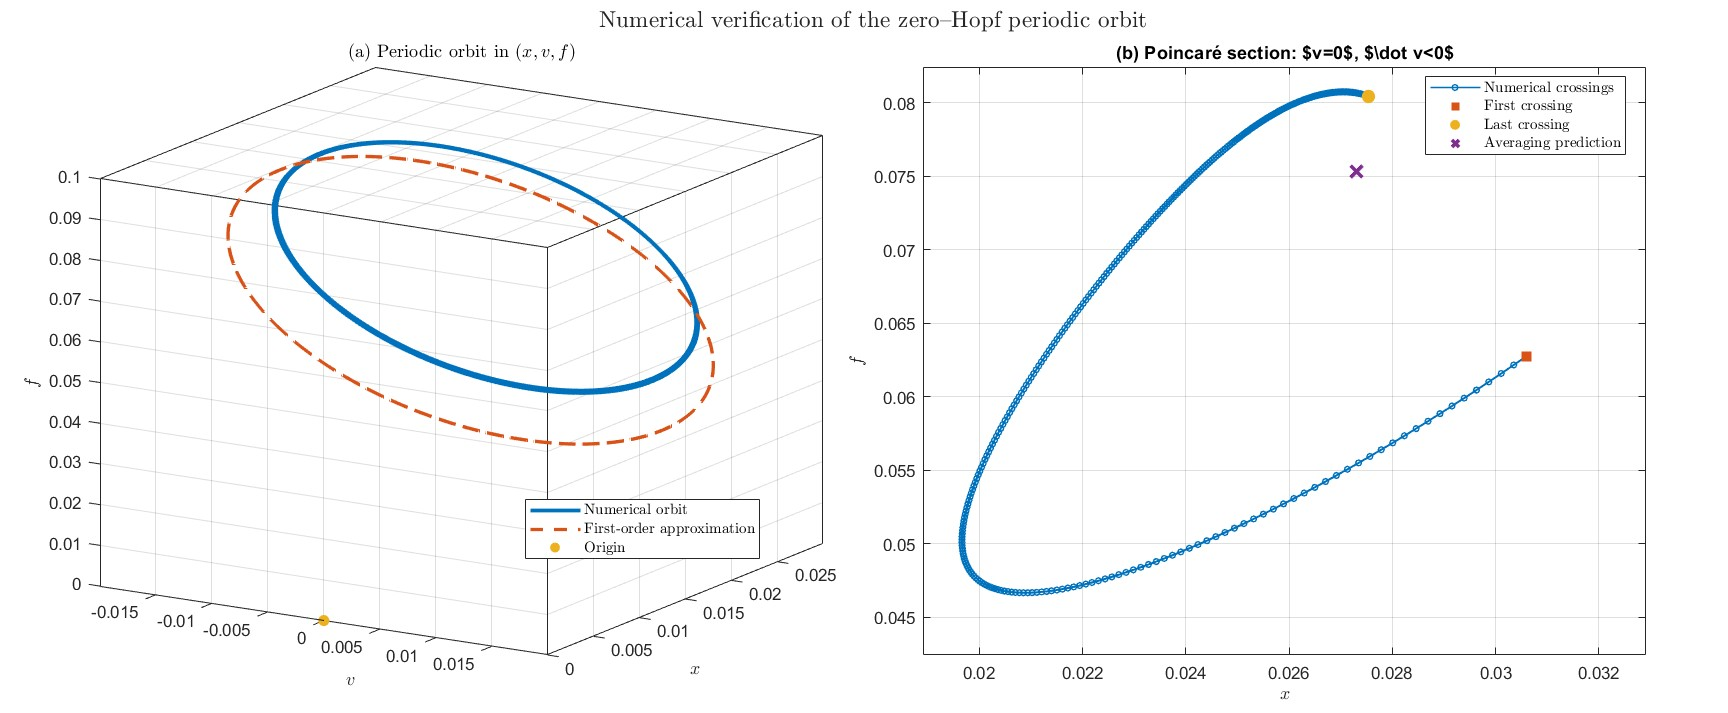
\includegraphics[width=\textwidth]
    {ZH}
    \caption{Numerical verification of the periodic orbit bifurcating
    from the zero--Hopf equilibrium for
    $\omega_0=2$, $\tau=1$, $\kappa=1$, $d=0.2$,
    $g_1=-0.2$, $k_1=1$, and $\varepsilon=0.02$.
    Panel~(a) compares the periodic orbit obtained by numerical
    integration of the full oscillator--actuator system with its
    first-order approximation derived by averaging. Panel~(b) shows
    successive intersections of the numerical trajectory with the
    Poincaré section $v=0$, $\dot v<0$. The convergence of these
    intersections toward a single point provides numerical evidence
    for the orbital asymptotic stability predicted by
    $\varepsilon g_1<0$.}
    \label{fig:numerical-verification}
\end{figure}

\subsection{Polar-coordinate formulation}
We now construct a real linear transformation that puts the linear part
of system \eqref{eq:model} at the critical zero--Hopf parameter values

\[
g=g_*:=d+\frac{1}{\tau},
\qquad
k_s=k_{s*}:=\omega_0^2
\]

into canonical form. 
At the critical parameter values, the linearization of
\eqref{eq:model} at the origin is

\begin{equation}
\label{eq:A0-general}
A_0=
\begin{pmatrix}
0 & 1 & 0\\[1mm]
-\omega_0^2 & \dfrac{1}{\tau} & 1\\[2mm]
\dfrac{\omega_0^2}{\tau} & 0 & -\dfrac{1}{\tau}
\end{pmatrix}.
\end{equation}
Hence, the eigenvalues of $A_0$ are

\[
\lambda_1=0,
\qquad
\lambda_{2,3}=\pm i\Omega.
\]

We seek a real nonsingular matrix $P$ such that

\begin{equation}
\label{eq:similarity-objective}
P^{-1}A_0P
=
J,
\qquad
J=
\begin{pmatrix}
0&-\Omega&0\\
\Omega&0&0\\
0&0&0
\end{pmatrix}.
\end{equation}

If

\[
P=
\begin{pmatrix}
p_1&p_2&p_3
\end{pmatrix},
\]

then its columns must satisfy

\begin{equation}
\label{eq:column-relations}
A_0p_1=\Omega p_2,
\qquad
A_0p_2=-\Omega p_1,
\qquad
A_0p_3=0.
\end{equation}
Then we have
\begin{equation}
\label{eq:P-general}
P=
\begin{pmatrix}
p_1&p_2&p_3
\end{pmatrix}
=
\begin{pmatrix}
1&0&\dfrac{1}{\omega_0^2}\\[3mm]
0&-\Omega&0\\[2mm]
\dfrac{1}{\tau^2}&
\dfrac{\Omega}{\tau}&1
\end{pmatrix}.
\end{equation}

Its determinant is
\begin{equation}
\label{eq:detP-general}
\det P
=
-\frac{\Omega^3}{\omega_0^2}
\neq0.
\end{equation}
Thus, $P$ is nonsingular.

We introduce the real zero--Hopf coordinates $(X,Y,Z)$ by

\begin{equation}
\label{eq:change-matrix-form}
\begin{pmatrix}
x\\v\\f
\end{pmatrix}
=
P
\begin{pmatrix}
X\\Y\\Z
\end{pmatrix}.
\end{equation}

Using \eqref{eq:P-general}, this transformation is 
\begin{equation}
\label{eq:change-general}
\begin{aligned}
x&=X+\frac{Z}{\omega_0^2},\\[2mm]
v&=-\Omega Y,\\[2mm]
f&=\frac{X}{\tau^2}
+\frac{\Omega}{\tau}Y+Z.
\end{aligned}
\end{equation}

Thus the system
\eqref{eq:model} in the new variables $(X, Y, Z)$ becomes 
\begin{equation}
\label{eq:expanded-XYZ-system}
\begin{aligned}
\dot X
={}&
-\Omega Y
+\varepsilon
\left[
\frac{g_1}{\Omega\tau}Y
-\frac{k_1}{\Omega^2\tau}X
-\frac{k_1}{\Omega^2\omega_0^2\tau}Z
\right]
\\
&+
\frac{\kappa}{\Omega^2\tau}X^2
+\frac{2\kappa}{\Omega^2\omega_0^2\tau}XZ
+\frac{\kappa}{\Omega^2\omega_0^4\tau}Z^2,
\\[2mm]
\dot Y
={}&
\Omega X+\varepsilon g_1Y,
\\[2mm]
\dot Z
={}&
\varepsilon
\left[
-\frac{g_1\omega_0^2}{\Omega\tau}Y
+\frac{k_1\omega_0^2}{\Omega^2\tau}X
+\frac{k_1}{\Omega^2\tau}Z
\right]
\\
&-
\frac{\kappa\omega_0^2}{\Omega^2\tau}X^2
-\frac{2\kappa}{\Omega^2\tau}XZ
-\frac{\kappa}{\Omega^2\omega_0^2\tau}Z^2.
\end{aligned}
\end{equation}
We now transform this system into
polar coordinates in order to apply the first-order averaging method.

The motion in the $(X,Y)$-plane is therefore a harmonic rotation with
angular velocity $\Omega$. Since we seek periodic solutions
bifurcating from the zero--Hopf equilibrium, whose amplitudes are of
order $O(\varepsilon)$, we introduce the scaled polar coordinates

\begin{equation}
\label{eq:polar-transformation}
X=\varepsilon r\cos\theta,
\qquad
Y=\varepsilon r\sin\theta,
\qquad
Z=\varepsilon u,
\end{equation}
where
$
r\ge0,
u\in\mathbb R,
$ and 
$\theta\in\mathbb S^1.
$

The scaling is chosen so that the periodic solutions obtained below
remain at a distance $O(|\varepsilon|)$ from the equilibrium, which is
the natural size predicted by averaging near a zero--Hopf point.

By taking $\theta$ as a new independent variable the new differential system in new variables $(r,\theta)$ as the standard first-order averaging form
\begin{equation}
\label{eq:standard-averaging-form}
\begin{aligned}
r'
&=
\varepsilon
F_{11}(\theta,r,u)
+
O(\varepsilon^2),
\\[2mm]
u'
&=
\varepsilon
F_{12}(\theta,r,u)
+
O(\varepsilon^2),
\end{aligned}
\end{equation}

where

\begin{equation}
\label{eq:F11F12}
F_{11}
=
\frac{P\cos\theta+Q\sin\theta}{\Omega},
\qquad
F_{12}
=
\frac{R}{\Omega}.
\end{equation}
To simplify the notation, 
\begin{equation}
\label{eq:PQR}
\begin{aligned}
P(r,u,\theta)
&=
\frac{g_1r\sin\theta}{\Omega\tau}
-\frac{k_1}{\Omega^2\tau}H
+\frac{\kappa}{\Omega^2\tau}H^2,
\\[2mm]
Q(r,u,\theta)
&=
g_1r\sin\theta,
\\[2mm]
R(r,u,\theta)
&=
-\frac{g_1\omega_0^2r\sin\theta}
{\Omega\tau}
+\frac{k_1\omega_0^2}
{\Omega^2\tau}H
-\frac{\kappa\omega_0^2}
{\Omega^2\tau}H^2.
\end{aligned}
\end{equation}

The functions $F_{11}$ and $F_{12}$ are $2\pi$-periodic in the angular
variable $\theta$. Hence, system
\eqref{eq:standard-averaging-form} is in the standard form required for
the application of the first-order averaging theorem.

\subsection{First-order averaging}

The system \eqref{eq:standard-averaging-form} has the form

\begin{equation}
\label{eq:standard-averaging}
\begin{aligned}
r'
&=
\varepsilon
F_{11}(\theta,r,u)
+
O(\varepsilon^2),
\\
u'
&=
\varepsilon
F_{12}(\theta,r,u)
+
O(\varepsilon^2),
\end{aligned}
\end{equation}

where the functions $F_{11}$ and $F_{12}$ are continuously
differentiable and $2\pi$-periodic with respect to the angular
variable $\theta$.

The first averaged function associated with
\eqref{eq:standard-averaging} is defined by

\begin{equation}
\label{eq:first-averaged-definition}
f_1(r,u)
=
\begin{pmatrix}
f_{11}(r,u)
\\[2mm]
f_{12}(r,u)
\end{pmatrix},
\end{equation}

where

\begin{equation}
\label{eq:first-average-integral}
\boxed{
f_1(r,u)
=
\int_0^{2\pi}
\begin{pmatrix}
F_{11}(\theta,r,u)
\\[2mm]
F_{12}(\theta,r,u)
\end{pmatrix}
\,d\theta.
}
\end{equation}

The existence of periodic solutions is a direct consequence of the
first-order averaging theorem.

\begin{theorem}[First-order averaging]
\label{thm:averaging}

Consider the differential system

\[
x'
=
\varepsilon F(\theta,x)
+
O(\varepsilon^2),
\]

where $F(\theta,x)$ is continuously differentiable and
$2\pi$-periodic in $\theta$.

Suppose that the averaged function

\[
f(x)
=
\int_0^{2\pi}
F(\theta,x)\,d\theta
\]

has a zero $x_0$ satisfying

\[
f(x_0)=0,
\qquad
\det Df(x_0)\neq0.
\]

Then, for all sufficiently small $|\varepsilon|>0$, there exists a
unique $2\pi$-periodic solution

\[
x(\theta,\varepsilon)
=
x_0+O(\varepsilon),
\]

of the averaged system. Moreover, this periodic solution corresponds
to a periodic solution of the original differential system.
\end{theorem}

Therefore, our task reduces to computing the averaged function
$f_1(r,u)$, determining its zeros, and verifying that the Jacobian
matrix is nonsingular at the corresponding solution.

To evaluate the integrals, we use the identities

\[
\int_0^{2\pi}\sin\theta\,d\theta
=
\int_0^{2\pi}\cos\theta\,d\theta
=
\int_0^{2\pi}\sin\theta\cos\theta\,d\theta
=
0,
\]

\[
\int_0^{2\pi}\cos^3\theta\,d\theta
=
0,
\]

and

\[
\int_0^{2\pi}\sin^2\theta\,d\theta
=
\int_0^{2\pi}\cos^2\theta\,d\theta
=
\pi.
\]

Using the expressions for $P$, $Q$, and $R$ in
\eqref{eq:PQR}, the functions appearing in
\eqref{eq:standard-averaging-form} are

\begin{equation}
\label{eq:F11-unexpanded}
\boxed{
\begin{aligned}
F_{11}
={}&
\frac{g_1r\sin\theta\cos\theta}{\Omega^2\tau}
+\frac{g_1r\sin^2\theta}{\Omega}
\\
&
-\frac{k_1\cos\theta}{\Omega^3\tau}
\left(
r\cos\theta+\frac{u}{\omega_0^2}
\right)
\\
&
+\frac{\kappa\cos\theta}{\Omega^3\tau}
\left(
r\cos\theta+\frac{u}{\omega_0^2}
\right)^2,
\end{aligned}}
\end{equation}

and

\begin{equation}
\label{eq:F12-unexpanded}
\boxed{
\begin{aligned}
F_{12}
={}&
-\frac{g_1\omega_0^2r\sin\theta}
{\Omega^2\tau}
\\
&
+\frac{k_1\omega_0^2}
{\Omega^3\tau}
\left(
r\cos\theta+\frac{u}{\omega_0^2}
\right)
\\
&
-\frac{\kappa\omega_0^2}
{\Omega^3\tau}
\left(
r\cos\theta+\frac{u}{\omega_0^2}
\right)^2.
\end{aligned}}
\end{equation}

Expanding the quadratic terms gives

\begin{equation}
\label{eq:F11-expanded}
\boxed{
\begin{aligned}
F_{11}
={}&
\frac{g_1r\sin\theta\cos\theta}{\Omega^2\tau}
+\frac{g_1r\sin^2\theta}{\Omega}
-\frac{k_1r\cos^2\theta}{\Omega^3\tau}
\\
&
-\frac{k_1u\cos\theta}
{\Omega^3\tau\omega_0^2}
+\frac{\kappa r^2\cos^3\theta}
{\Omega^3\tau}
\\
&
+\frac{2\kappa ru\cos^2\theta}
{\Omega^3\tau\omega_0^2}
+\frac{\kappa u^2\cos\theta}
{\Omega^3\tau\omega_0^4},
\end{aligned}}
\end{equation}

and

\begin{equation}
\label{eq:F12-expanded}
\boxed{
\begin{aligned}
F_{12}
={}&
-\frac{g_1\omega_0^2r\sin\theta}
{\Omega^2\tau}
+\frac{k_1\omega_0^2r\cos\theta}
{\Omega^3\tau}
+\frac{k_1u}{\Omega^3\tau}
\\
&
-\frac{\kappa\omega_0^2r^2\cos^2\theta}
{\Omega^3\tau}
-\frac{2\kappa ru\cos\theta}
{\Omega^3\tau}
-\frac{\kappa u^2}
{\Omega^3\tau\omega_0^2}.
\end{aligned}}
\end{equation}

Integrating \eqref{eq:F11-expanded} over one period yields

\begin{align}
f_{11}(r,u)
&=
\frac{\pi r}{\Omega}
\left(
g_1
-
\frac{k_1}{\Omega^2\tau}
+
\frac{2\kappa u}
{\Omega^2\tau\omega_0^2}
\right).
\end{align}

Similarly,

\begin{align}
f_{12}(r,u)
&=
\frac{\pi}{\Omega^3\tau}
\left(
2k_1u
-
\kappa\omega_0^2r^2
-
\frac{2\kappa u^2}
{\omega_0^2}
\right).
\end{align}

Hence, the first averaged function is

\begin{equation}
\label{eq:first-averaged-function}
\boxed{
f_1(r,u)
=
\begin{pmatrix}
\dfrac{\pi r}{\Omega}
\left(
g_1
-\dfrac{k_1}{\Omega^2\tau}
+\dfrac{2\kappa u}
{\Omega^2\tau\omega_0^2}
\right)
\\[6mm]
\dfrac{\pi}{\Omega^3\tau}
\left(
2k_1u
-
\kappa\omega_0^2r^2
-
\dfrac{2\kappa u^2}
{\omega_0^2}
\right)
\end{pmatrix}.
}
\end{equation}

Unlike several classical zero--Hopf problems for which the first
averaged function vanishes identically and higher-order averaging is
required, the present oscillator--actuator model possesses a
nontrivial first averaged function. Consequently, first-order
averaging is sufficient to detect periodic solutions bifurcating from
the zero--Hopf equilibrium.

\subsection{Zeros of the first averaged function}

According to Theorem~\ref{thm:averaging}, the existence of periodic
solutions is determined by the zeros of the first averaged function
\eqref{eq:first-averaged-function}. We therefore seek all solutions of

\[
f_1(r,u)=0,
\qquad r>0,
\]

where the restriction $r>0$ excludes the equilibrium itself and
corresponds to genuine periodic oscillations.

Recall that

\begin{equation}
\label{eq:averaged-components}
\begin{aligned}
f_{11}(r,u)
&=
\frac{\pi r}{\Omega}
\left(
g_1
-\frac{k_1}{\Omega^2\tau}
+\frac{2\kappa u}
{\Omega^2\tau\omega_0^2}
\right),
\\[2mm]
f_{12}(r,u)
&=
\frac{\pi}{\Omega^3\tau}
\left(
2k_1u
-\kappa\omega_0^2r^2
-\frac{2\kappa u^2}{\omega_0^2}
\right).
\end{aligned}
\end{equation}

Since $r>0$, the first equation

\[
f_{11}(r,u)=0
\]

is equivalent to

\[
g_1
-
\frac{k_1}{\Omega^2\tau}
+
\frac{2\kappa u}
{\Omega^2\tau\omega_0^2}
=
0.
\]

Hence,

\begin{equation}
\label{eq:u0}
\boxed{
u_0
=
\frac{\omega_0^2}{2\kappa}
\left(
k_1-g_1\Omega^2\tau
\right).
}
\end{equation}

Substituting \eqref{eq:u0} into the second equation

\[
f_{12}(r,u)=0,
\]

gives

\[
2k_1u_0
-
\kappa\omega_0^2r^2
-
\frac{2\kappa u_0^2}{\omega_0^2}
=
0.
\]

After simplification,

\begin{equation}
\label{eq:r0-square}
\boxed{
r_0^2
=
\frac{
k_1^2-g_1^2\Omega^4\tau^2
}
{2\kappa^2}.
}
\end{equation}

Consequently,

\begin{equation}
\label{eq:r0}
\boxed{
r_0
=
\sqrt{
\frac{
k_1^2-g_1^2\Omega^4\tau^2
}
{2\kappa^2}
}.
}
\end{equation}

Therefore, a nontrivial zero exists if and only if

\begin{equation}
\label{eq:existence-condition}
\boxed{
k_1^2-g_1^2\Omega^4\tau^2>0.
}
\end{equation}

Under condition
\eqref{eq:existence-condition},
the averaged system possesses the isolated zero

\begin{equation}
\label{eq:averaged-zero}
\boxed{
(r_0,u_0)
=
\left(
\sqrt{
\frac{
k_1^2-g_1^2\Omega^4\tau^2
}
{2\kappa^2}
},
\;
\frac{\omega_0^2}{2\kappa}
\left(
k_1-g_1\Omega^2\tau
\right)
\right).
}
\end{equation}

Since $r_0>0$, this solution corresponds to a nontrivial oscillatory
state rather than to the equilibrium point.

%%%%%%%%%%%%%%%%%%%%%%%%%%%%%%%%%%%%%%%%%%%%%%%%%%%%%%%%%%%%%%%

\subsection{Nondegeneracy of the averaged zero}

To apply Theorem~\ref{thm:averaging}, it remains to verify that the
zero \eqref{eq:averaged-zero} is nondegenerate.

The Jacobian matrix of the averaged function is

\[
Df_1(r,u)
=
\begin{pmatrix}
\dfrac{\partial f_{11}}{\partial r}
&
\dfrac{\partial f_{11}}{\partial u}
\\[4mm]
\dfrac{\partial f_{12}}{\partial r}
&
\dfrac{\partial f_{12}}{\partial u}
\end{pmatrix}.
\]

Differentiating \eqref{eq:averaged-components} yields

\begin{align}
\frac{\partial f_{11}}{\partial r}
&=
\frac{\pi}{\Omega}
\left(
g_1
-\frac{k_1}{\Omega^2\tau}
+\frac{2\kappa u}
{\Omega^2\tau\omega_0^2}
\right),
\nonumber\\[2mm]
\frac{\partial f_{11}}{\partial u}
&=
\frac{2\pi\kappa r}
{\Omega^3\tau\omega_0^2},
\nonumber\\[2mm]
\frac{\partial f_{12}}{\partial r}
&=
-\frac{2\pi\kappa\omega_0^2r}
{\Omega^3\tau},
\nonumber\\[2mm]
\frac{\partial f_{12}}{\partial u}
&=
\frac{\pi}{\Omega^3\tau}
\left(
2k_1
-\frac{4\kappa u}{\omega_0^2}
\right).
\label{eq:partial-derivatives}
\end{align}

Evaluating these derivatives at the zero
$(r_0,u_0)$ and using
\eqref{eq:u0} gives

\[
\left.
\frac{\partial f_{11}}{\partial r}
\right|_{(r_0,u_0)}
=
0,
\]

and

\[
\left.
\frac{\partial f_{12}}{\partial u}
\right|_{(r_0,u_0)}
=
\frac{2\pi g_1}{\Omega}.
\]

Hence,

\begin{equation}
\label{eq:jacobian}
\boxed{
Df_1(r_0,u_0)
=
\begin{pmatrix}
0
&
\dfrac{2\pi\kappa r_0}
{\Omega^3\tau\omega_0^2}
\\[5mm]
-\dfrac{2\pi\kappa\omega_0^2r_0}
{\Omega^3\tau}
&
\dfrac{2\pi g_1}{\Omega}
\end{pmatrix}.
}
\end{equation}

Its determinant is

\begin{align}
\det Df_1(r_0,u_0)
&=
\frac{
4\pi^2\kappa^2r_0^2
}
{\Omega^6\tau^2}
\nonumber\\
&=
\frac{
2\pi^2
\left(
k_1^2-g_1^2\Omega^4\tau^2
\right)
}
{\Omega^6\tau^2}.
\end{align}

Therefore,

\begin{equation}
\label{eq:jacobian-determinant}
\boxed{
\det Df_1(r_0,u_0)
=
\frac{
2\pi^2
\left(
k_1^2-g_1^2\Omega^4\tau^2
\right)
}
{\Omega^6\tau^2}
>0.
}
\end{equation}

Condition \eqref{eq:existence-condition} therefore guarantees that the
zero \eqref{eq:averaged-zero} is isolated and nondegenerate.
Consequently, all hypotheses of
Theorem~\ref{thm:averaging} are satisfied.

\subsection{Existence and stability of the periodic orbit}

Since all the hypotheses of Theorem~\ref{thm:averaging} are satisfied,
the averaged system \eqref{eq:standard-averaging-form} possesses a
$2\pi$-periodic solution satisfying

\[
(r(\theta,\varepsilon),u(\theta,\varepsilon))
=
(r_0,u_0)+O(\varepsilon),
\]

where $(r_0,u_0)$ is given by
\eqref{eq:averaged-zero}.

The averaging theorem implies that this periodic solution corresponds
to a periodic solution of the original differential system
\eqref{eq:perturbed-model}. Consequently, for all sufficiently small
$|\varepsilon|>0$, system \eqref{eq:perturbed-model} possesses a
periodic orbit whose amplitude is $O(|\varepsilon|)$.

%%%%%%%%%%%%%%%%%%%%%%%%%%%%%%%%%%%%%%%%%%%%%%%%%%%%%%%%%%%%%%%

\subsubsection*{Poincaré-map interpretation}

The existence result can be interpreted in terms of the Poincaré map.

Let

\[
\Pi_\varepsilon:\mathbb{R}^2\rightarrow\mathbb{R}^2
\]

denote the Poincaré map associated with one complete revolution
$\theta\mapsto\theta+2\pi$ of the reduced system
\eqref{eq:standard-averaging-form}. Standard averaging theory gives the
expansion

\begin{equation}
\label{eq:poincare-expansion}
\boxed{
\Pi_\varepsilon(z)
=
z
+
\varepsilon f_1(z)
+
O(\varepsilon^2),
}
\end{equation}

where

\[
z=(r,u),
\]

and $f_1$ is the first averaged function
\eqref{eq:first-averaged-function}.

Since

\[
f_1(r_0,u_0)=0,
\]

equation \eqref{eq:poincare-expansion} implies that

\[
\Pi_\varepsilon(r_0,u_0)
=
(r_0,u_0)
+
O(\varepsilon^2).
\]

Because

\[
\det Df_1(r_0,u_0)\neq0,
\]

the Implicit Function Theorem guarantees the existence of a unique
fixed point

\[
(r_\varepsilon,u_\varepsilon)
=
(r_0,u_0)+O(\varepsilon)
\]

of the Poincaré map. This fixed point corresponds precisely to the
periodic orbit obtained from the averaging theorem.

%%%%%%%%%%%%%%%%%%%%%%%%%%%%%%%%%%%%%%%%%%%%%%%%%%%%%%%%%%%%%%%

\subsubsection*{Stability}

The derivative of the Poincaré map satisfies

\begin{equation}
\label{eq:poincare-derivative}
\boxed{
D\Pi_\varepsilon(r_\varepsilon,u_\varepsilon)
=
I
+
\varepsilon
Df_1(r_0,u_0)
+
O(\varepsilon^2),
}
\end{equation}

where

\[
Df_1(r_0,u_0)
=
\begin{pmatrix}
0
&
\dfrac{2\pi\kappa r_0}
{\Omega^3\tau\omega_0^2}
\\[5mm]
-\dfrac{2\pi\kappa\omega_0^2r_0}
{\Omega^3\tau}
&
\dfrac{2\pi g_1}{\Omega}
\end{pmatrix}.
\]

Its trace and determinant are

\begin{equation}
\label{eq:trace-det}
\boxed{
\operatorname{tr}Df_1(r_0,u_0)
=
\frac{2\pi g_1}{\Omega},
\qquad
\det Df_1(r_0,u_0)
=
\frac{
2\pi^2
\left(
k_1^2-g_1^2\Omega^4\tau^2
\right)
}
{\Omega^6\tau^2}.
}
\end{equation}

The eigenvalues of $Df_1(r_0,u_0)$ are

\begin{equation}
\label{eq:averaged-eigenvalues}
\boxed{
\lambda_\pm
=
\frac{\pi g_1}{\Omega}
\pm
\frac{\pi}
{\Omega^3\tau}
\sqrt{
3g_1^2\Omega^4\tau^2
-
2k_1^2
}.
}
\end{equation}

Consequently, the two nontrivial Floquet multipliers of the periodic
orbit satisfy

\begin{equation}
\label{eq:floquet-expansion}
\boxed{
\mu_i
=
1+\varepsilon\lambda_i
+
O(\varepsilon^2),
\qquad
i=1,2.
}
\end{equation}

(The third Floquet multiplier is identically equal to one because it
corresponds to the direction tangent to the periodic orbit.)

If

\[
3g_1^2\Omega^4\tau^2
<
2k_1^2,
\]

the eigenvalues form a complex conjugate pair with

\[
\operatorname{Re}\lambda_\pm
=
\frac{\pi g_1}{\Omega}.
\]

Otherwise, the eigenvalues are real. Since

\[
\det Df_1(r_0,u_0)>0,
\]

they necessarily have the same sign, which is determined by the trace.

Therefore,

\[
\operatorname{Re}\lambda_i<0
\quad\Longleftrightarrow\quad
g_1<0,
\]

and

\[
\operatorname{Re}\lambda_i>0
\quad\Longleftrightarrow\quad
g_1>0.
\]

Since

\[
\mu_i
=
1+\varepsilon\lambda_i+O(\varepsilon^2),
\]

the periodic orbit is asymptotically stable whenever

\[
\varepsilon g_1<0,
\]

and unstable whenever

\[
\varepsilon g_1>0.
\]

Hence we obtain the following result.

The averaged system possesses the simple zero
$(r_0,u_0)$, where

\[
r_0=
\sqrt{\frac{k_1^2-g_1^2\Omega^4\tau^2}{2\kappa^2}},
\qquad
u_0=
\frac{\omega_0^2}{2\kappa}
(k_1-g_1\Omega^2\tau),
\]

and

\[
\det Df_1(r_0,u_0)\neq0.
\]

Therefore, all the hypotheses of the first-order averaging theorem are
satisfied. Consequently, Theorem~\ref{thm:periodic-orbit} follows.
\subsection{Approximation of the bifurcating periodic orbit}

The periodic solution obtained in Theorem~\ref{thm:periodic-orbit} is
expressed in the variables $(r,\theta,u)$.
To recover the periodic orbit in the original coordinates, we first
return to the time variable.

From \eqref{eq:rtu-time-system},

\[
\dot\theta
=
\Omega
+
O(\varepsilon),
\]

and therefore

\begin{equation}
\label{eq:theta-time}
\boxed{
\theta(t,\varepsilon)
=
\Omega t+\theta_0+O(\varepsilon),
}
\end{equation}

where $\theta_0$ is an arbitrary initial phase.

Moreover,

\[
r(t,\varepsilon)
=
r_0+O(\varepsilon),
\qquad
u(t,\varepsilon)
=
u_0+O(\varepsilon),
\]

where

\[
r_0
=
\sqrt{
\frac{
k_1^2-g_1^2\Omega^4\tau^2
}
{2\kappa^2}
},
\qquad
u_0
=
\frac{\omega_0^2}{2\kappa}
\left(
k_1-g_1\Omega^2\tau
\right).
\]

Consequently, the leading-order period is

\begin{equation}
\label{eq:period}
\boxed{
T_\varepsilon
=
\frac{2\pi}{\Omega}
+
O(\varepsilon).
}
\end{equation}

%%%%%%%%%%%%%%%%%%%%%%%%%%%%%%%%%%%%%%%%%%%%%%%%%%%%%%%%%%%%%%%

\subsubsection*{Reconstruction in the $(X,Y,Z)$ coordinates}

Using the polar transformation

\[
X=\varepsilon r\cos\theta,
\qquad
Y=\varepsilon r\sin\theta,
\qquad
Z=\varepsilon u,
\]

together with \eqref{eq:theta-time}, we obtain

\begin{equation}
\label{eq:XYZ-periodic}
\boxed{
\begin{aligned}
X(t,\varepsilon)
&=
\varepsilon r_0\cos(\Omega t+\theta_0)
+
O(\varepsilon^2),
\\[2mm]
Y(t,\varepsilon)
&=
\varepsilon r_0\sin(\Omega t+\theta_0)
+
O(\varepsilon^2),
\\[2mm]
Z(t,\varepsilon)
&=
\varepsilon u_0
+
O(\varepsilon^2).
\end{aligned}}
\end{equation}

Hence, to leading order, the periodic orbit is a circle of radius
$\varepsilon r_0$ in the $(X,Y)$-plane, translated by
$\varepsilon u_0$ in the $Z$-direction.

%%%%%%%%%%%%%%%%%%%%%%%%%%%%%%%%%%%%%%%%%%%%%%%%%%%%%%%%%%%%%%%

\subsubsection*{Reconstruction in the original variables}

Finally, recall that the inverse linear transformation is

\[
x
=
X+\frac{Z}{\omega_0^2},
\qquad
v
=
-\Omega Y,
\qquad
f
=
\frac{X}{\tau^2}
+\frac{\Omega}{\tau}Y
+Z.
\]

Substituting \eqref{eq:XYZ-periodic} yields

\begin{equation}
\label{eq:original-periodic-orbit}
\boxed{
\begin{aligned}
x(t,\varepsilon)
={}&
\varepsilon
\left(
r_0\cos(\Omega t+\theta_0)
+
\frac{u_0}{\omega_0^2}
\right)
+
O(\varepsilon^2),
\\[2mm]
v(t,\varepsilon)
={}&
-\varepsilon\Omega r_0
\sin(\Omega t+\theta_0)
+
O(\varepsilon^2),
\\[2mm]
f(t,\varepsilon)
={}&
\varepsilon
\left(
\frac{r_0}{\tau^2}
\cos(\Omega t+\theta_0)
+
\frac{\Omega r_0}{\tau}
\sin(\Omega t+\theta_0)
+
u_0
\right)
+
O(\varepsilon^2).
\end{aligned}}
\end{equation}

Substituting the explicit expressions for $r_0$ and $u_0$, the
leading-order approximation of the bifurcating periodic orbit becomes

\begin{equation}
\label{eq:explicit-periodic-orbit}
\boxed{
\begin{aligned}
x(t,\varepsilon)
={}&
\varepsilon
\sqrt{
\frac{
k_1^2-g_1^2\Omega^4\tau^2
}
{2\kappa^2}
}
\cos(\Omega t+\theta_0)
\\
&
+
\frac{\varepsilon}{2\kappa}
\left(
k_1-g_1\Omega^2\tau
\right)
+
O(\varepsilon^2),
\\[3mm]
v(t,\varepsilon)
={}&
-\varepsilon\Omega
\sqrt{
\frac{
k_1^2-g_1^2\Omega^4\tau^2
}
{2\kappa^2}
}
\sin(\Omega t+\theta_0)
+
O(\varepsilon^2),
\\[3mm]
f(t,\varepsilon)
={}&
\frac{\varepsilon}{\tau^2}
\sqrt{
\frac{
k_1^2-g_1^2\Omega^4\tau^2
}
{2\kappa^2}
}
\cos(\Omega t+\theta_0)
\\
&
+
\frac{\varepsilon\Omega}{\tau}
\sqrt{
\frac{
k_1^2-g_1^2\Omega^4\tau^2
}
{2\kappa^2}
}
\sin(\Omega t+\theta_0)
\\
&
+
\frac{\varepsilon\omega_0^2}{2\kappa}
\left(
k_1-g_1\Omega^2\tau
\right)
+
O(\varepsilon^2).
\end{aligned}}
\end{equation}

Therefore, whenever

\[
k_1^2-g_1^2\Omega^4\tau^2>0,
\]

a family of periodic solutions bifurcates from the zero--Hopf
equilibrium. The amplitude of the oscillation is proportional to
$|\varepsilon|$, the leading angular frequency is $\Omega$, and the
leading period is $2\pi/\Omega$. The stability of the periodic orbit is
determined by the sign of $\varepsilon g_1$, in accordance with
Theorem~\ref{thm:periodic-orbit}.




%\section*{Acknowledgments}
%[Funding, collaborations]

\bibliographystyle{plain}
\bibliography{bibliography}
%\printbibliography




\end{document}
